\documentclass{article}%
\usepackage[T1]{fontenc}%
\usepackage[utf8]{inputenc}%
\usepackage{lmodern}%
\usepackage{textcomp}%
\usepackage{lastpage}%
\usepackage[head=40pt,margin=0.5in,bottom=0.6in]{geometry}%
\usepackage{graphicx}%
%
\title{\textbf{Reportan cierre en la carretera Panamericana por protesta vecinal}}%
\author{EL NACIONAL WEB}%
\date{27/09/2018}%
%
\begin{document}%
\normalsize%
\maketitle%
\textbf{URL: }%
http://www.el{-}nacional.com/noticias/protestas/reportan{-}cierre{-}carretera{-}panamericana{-}por{-}protesta{-}vecinal\_253428\newline%
%
\textbf{Periodico: }%
EN, %
ID: %
253428, %
Seccion: %
Protestas\newline%
%
\textbf{Palabras Claves: }%
Sociedad\newline%
%
\textbf{Derecho: }%
2.8, %
Otros Derechos: %
, %
Sub Derechos: %
2.8.1\newline%
%
\textbf{EP: }%
SI\newline%
\newline%
%
\textbf{\textit{Habitantes del estado Miranda protestan a la altura del distribuidor Los Cerritos en exigencia de servicios públicos~}}%
\newline%
\newline%
%
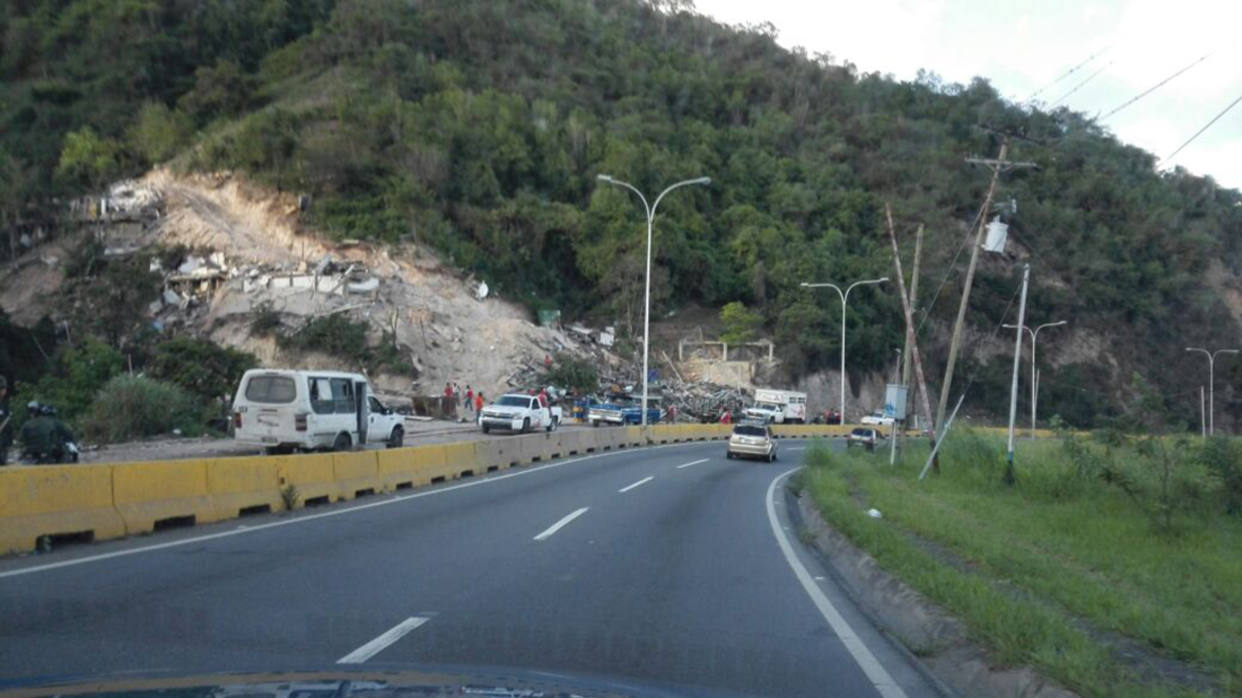
\includegraphics[width=300px]{13.jpg}%
\newline%
%
Vecinos del kilómetro 23 cerraron este jueves el acceso de vehículos en~la carretera Panamericana en rechazo a las fallas de servicios básicos en la entidad.%
\newline%
%
La información fue difundida~por el periodista Daniel Murolo, en Twitter.%
\newline%
%
Murolo señaló que las personas protestan a la altura del distribuidor Los Cerritos en exigencia del restablecimiento de los servicios públicos.%
\newline%
%
\end{document}